\chapter{Implementacija i korisničko sučelje}
		
		
		\section{Korištene tehnologije i alati}
			 
			 \noindent{Za izradu UML dijagrama korišten je alat Astah UML\footnote{\url{https://astah.net/products/astah-uml/}}}. Kao razvojno okruženje korišten je Visual Studio Code\footnote{\url{https://code.visualstudio.com/}}. Korišten je Git\footnote{\url{https://git-scm.com/}} kao sustav za upravljanje verzijama zajedno sa GitHub-om\footnote{\url{https://github.com/}} na kojem se nalazi udaljeni repozitorij projekta. Za potrebe izrade dokumentacije korišten je TeXstudio\footnote{\url{https://www.texstudio.org/}}, višeplatformski LaTeX editor otvorenog koda.\\
			 \indent{Za izradu backenda korišten je Django\footnote{\url{https://www.djangoproject.com/}}, besplatni radni okvir otvorenog koda za izradu web aplikacija u programskom jeziku Python\footnote{\url{https://www.python.org/}}. Za izradu frontenda korišten je React\footnote{\url{https://react.dev/}}, biblioteka napisana u programskom jeziku JavaScript\footnote{\url{https://developer.mozilla.org/en-US/docs/Web/JavaScript}}.}\\
			 \indent{Za potrebe baze podataka korišten je MongoDB\footnote{\url{https://www.mongodb.com/}}. Sama baza podataka nalazi se na udaljenom poslužitelju. Usluga koja omogućuje pristup, rad i postavljanje udaljene MongoDB baze podataka je MongoDB Atlas\footnote{\url{https://www.mongodb.com/atlas/database}}. Aplikacija je puštena u pogon na udaljenom poslužitelju pomoću usluge koje nudi Heroku\footnote{\url{https://www.heroku.com/}}. Heroku je cloud platforma kao usluga koja omogućuje puštanje u pogon aplikacija i podržava više programskih jezika.}\\
			 \indent{Aplikacija koristi Datamuse API\footnote{\url{https://www.datamuse.com/api/}} za pretraživanje i dohvat podataka o riječima. Za potrebe generiranja zvučnih datoteka izgovora riječi koristi Google Text-to-Speech API koji omogućuje sintezu govora iz teksta.\footnote{\url{https://cloud.google.com/text-to-speech/docs/reference/rest}}}\\
			 \indent{Za potrebe komunikacije tima korištene su aplikacije WhatsApp\footnote{\url{https://www.whatsapp.com/}} i Microsoft Teams\footnote{\url{https://www.microsoft.com/en-us/microsoft-teams/group-chat-software}}.
			 Za potrebe testiranja aplikacije osim ugrađene potpore za testiranje koju nudi Django korišten je i Selenium WebDriver\footnote{\url{https://www.selenium.dev/documentation/webdriver/}} koji omogućuje pisanje i automatizaciju testova za web aplikacije.}
			 
			
			\eject 
		
	
		\section{Ispitivanje programskog rješenja}
						
			\subsection{Ispitivanje komponenti}
			\noindent{Ispitivanje komponenti provedeno je korištenjem alata koje pruža radni okvir Django\footnote{\url{https://docs.djangoproject.com/en/5.0/topics/testing/tools/}}. U nastavku se za svaki ispitni slučaj definira ulaz, očekivani izlaz te kratak opis što je ispitano ispitnim slučajem. Rezultati izvođenja ispitnih slučajeva prikazani su na slici \ref{fig:test_results}.}\\
			\indent{S obzirom na to kako se koriste alati za ispitivanje u radnom okviru Django i način na koji funkcioniraju komponente koje se ispituju, za svaki ispitni slučaj vezana je metoda "setUp" koja će osigurati da prije izvođenja konkretnog ispitnog slučaja bude prisutno sve ono što je potrebno da se ispitni slučaj provede. Na sličan način, metoda "tearDown" osigurava da se nakon svakog provedenog ispitnog slučaja, obnovi stanje okoline prije njegovog izvršavanja. Zbog potpunosti i jasnoće, uz ispitne slučajeve priložene su metode "setUp" i "tearDown".}
				
			\indent{Nadalje, kao ulaz u ispitni slučaj, navode se samo podaci koji se smatraju relevantnima za dani ispitni slučaj. Npr., korisničko ime i lozinka testnog korisnika ne smatraju se relevantnima za ispitni slučaj koji ispituje ispravnost dodavanja riječi u rječnik, no njihovo postojanje je vidljivo u priloženom izvornom kodu.}
			
			
			\begin{figure}[H]
				\centering
				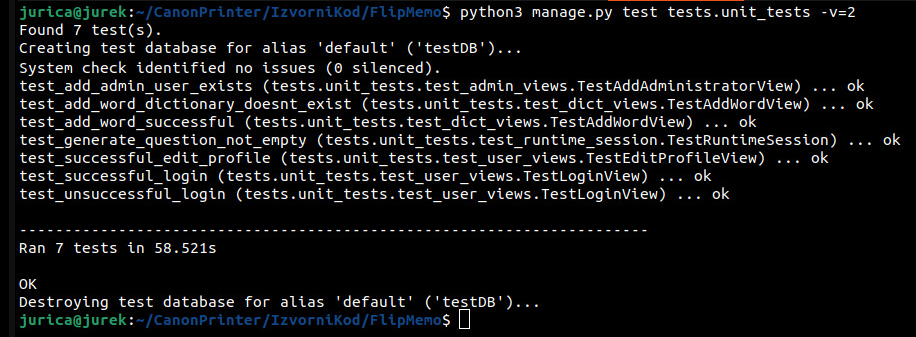
\includegraphics[width=\textwidth]{slike/test_results.png}
				\caption{Rezultati izvođenja ispitnih slučajeva}
				\label{fig:test_results}
			\end{figure}
			
			\eject
			
			\noindent{\textbf{Ispitivanje funkcionalnosti uređivanja profila}}\\
			\noindent{\textbf{Ulaz}: novo korisničko ime, novo ime i novo prezime\\\textbf{Očekivani izlaz:} novo korisničko ime, novo ime i novo prezime\\\textbf{Opis ispitnog slučaja:} ispituje se ispravno pohranjivanje novih podataka o profilu korisnika
			}
			
			
			\begin{figure}[H]
				\centering
				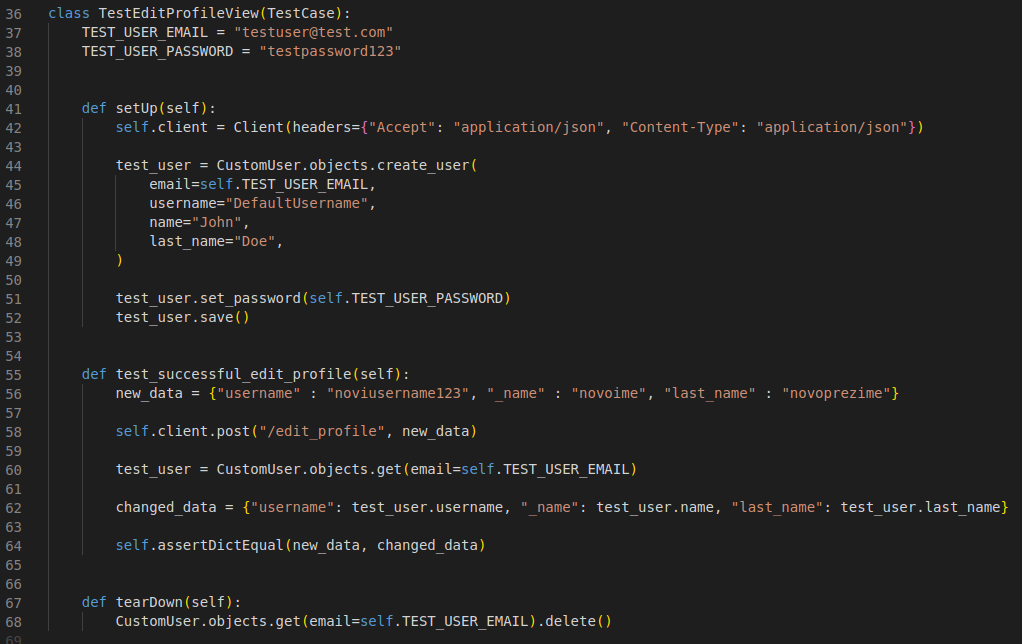
\includegraphics[width=\textwidth]{slike/test_successful_edit_profile.png}
				\caption{Ispitivanje funkcionalnosti uređivanja profila}
				\label{fig:test_successful_edit_profile1}
			\end{figure}
			
			\eject
			
			\noindent{\textbf{Ispitivanje dodavanja postojećeg korisnika kao novog administratora}}\\
			\noindent{\textbf{Ulaz}: email korisnika kojeg se želi dodati kao administratora\\\textbf{Očekivani izlaz:} korisnik nakon dodavanja ima privilegije administratora\\\textbf{Opis ispitnog slučaja:} ispituje se ispravnost funkcionalnosti dodavanja postojećeg korisnika kao administratora, uz pretpostavku da postojeći korisnik nije administrator
			}
			
			\begin{figure}[H]
				\centering
				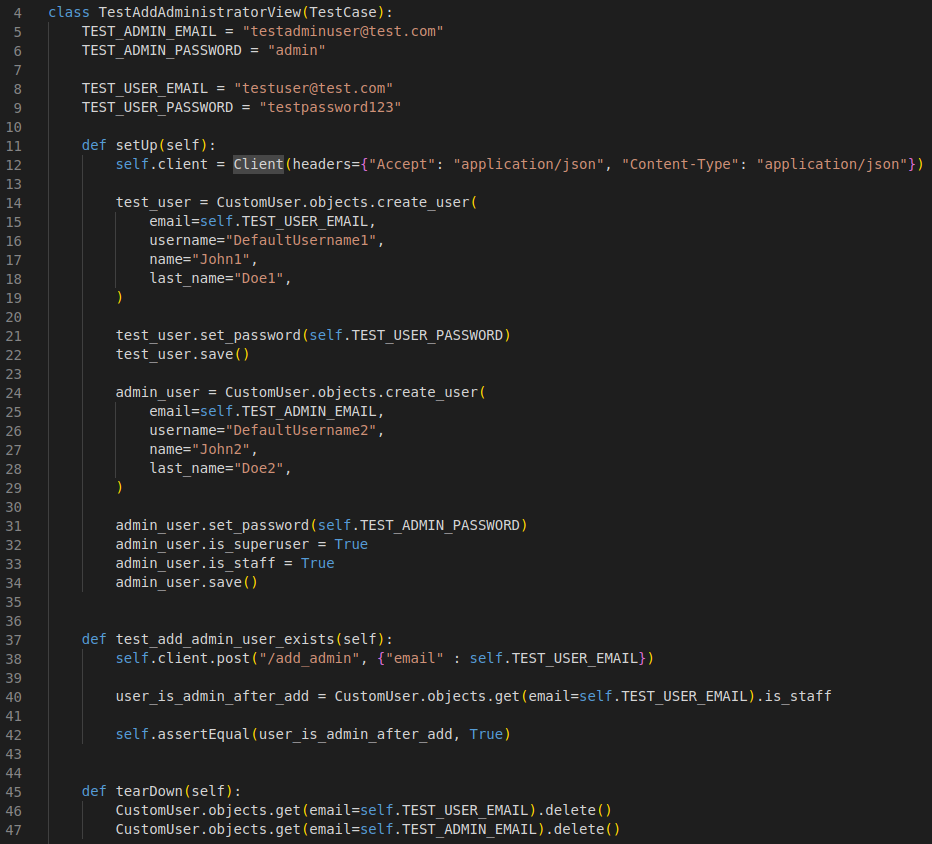
\includegraphics[width=\textwidth]{slike/test_add_admin_user_exists.png}
				\caption{Ispitivanje dodavanja postojećeg korisnika kao novog administratora}
				\label{fig:test_add_admin_user_exists}
			\end{figure}
		
		
			\eject
			
			\noindent{\textbf{Ispitivanje dodavanja nove riječi u rječnik}}\\
			\noindent{\textbf{Ulaz}: podaci o novoj riječi koja se želi dodati u rječnik, rječnik u koji se riječ dodaje\\\textbf{Očekivani izlaz:} riječ nakon dodavanja postoji i nalazi se u odabranom rječniku\\\textbf{Opis ispitnog slučaja:} ispituje se ispravnost funkcionalnosti dodavanja nove riječi u postojeći rječnik
			}
			
			\begin{figure}[H]
				\centering
				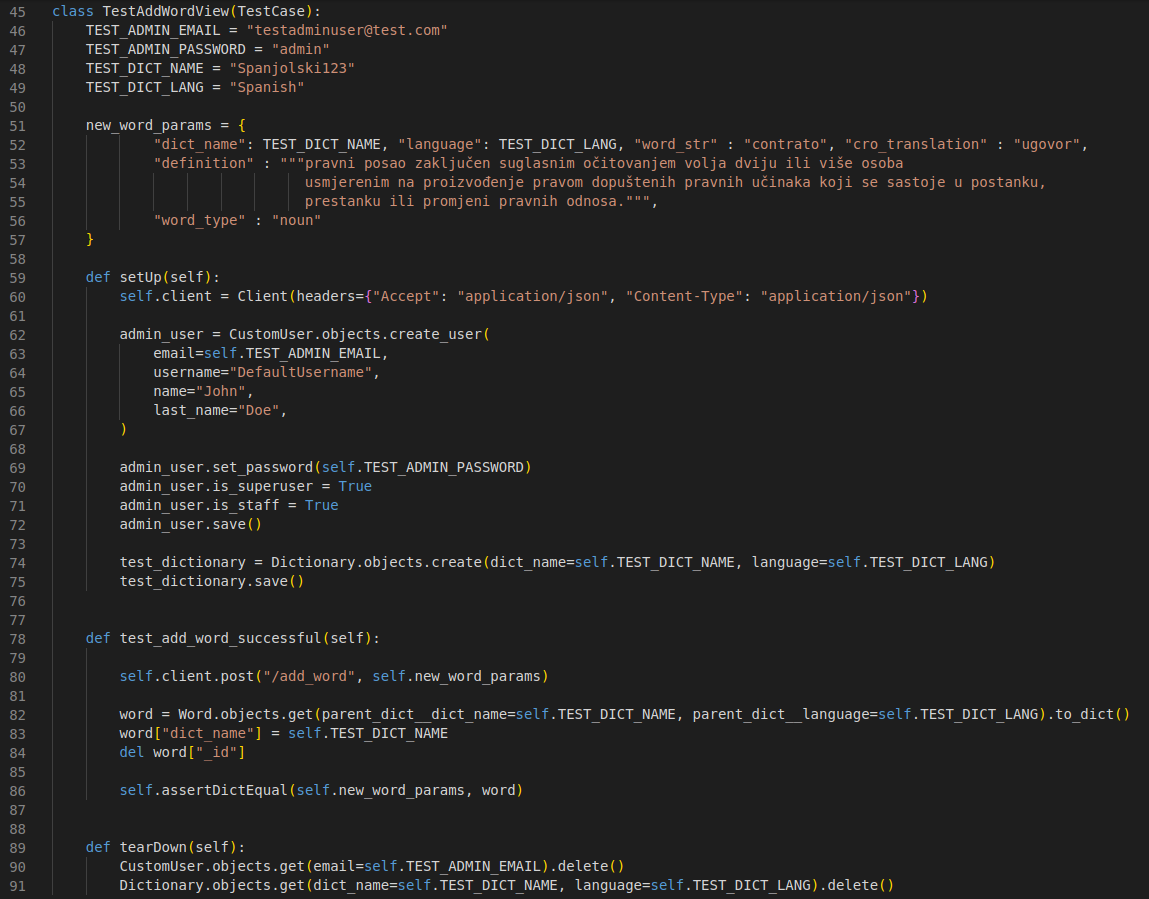
\includegraphics[width=\textwidth]{slike/test_add_word_successful.png}
				\caption{Ispitivanje dodavanja nove riječi u rječnik}
				\label{fig:test_add_word_successful}
			\end{figure}
		
		
			\eject
			
			\noindent{\textbf{Ispitivanje dodavanja nove riječi u nepostojeći rječnik}}\\
			\noindent{\textbf{Ulaz}: podaci o novoj riječi koja se želi dodati u rječnik, rječnik u koji se riječ dodaje\\\textbf{Očekivani izlaz:} greška koja opisuje da rječnik u koji se želi dodati nova riječ ne postoji\\\textbf{Opis ispitnog slučaja:} ispituje se ispravnost odgovora funkcionalnosti dodavanja riječi na situaciju u kojoj se riječ želi dodati u nepostojeći rječnik
			}
		
			\begin{figure}[H]
				\centering
				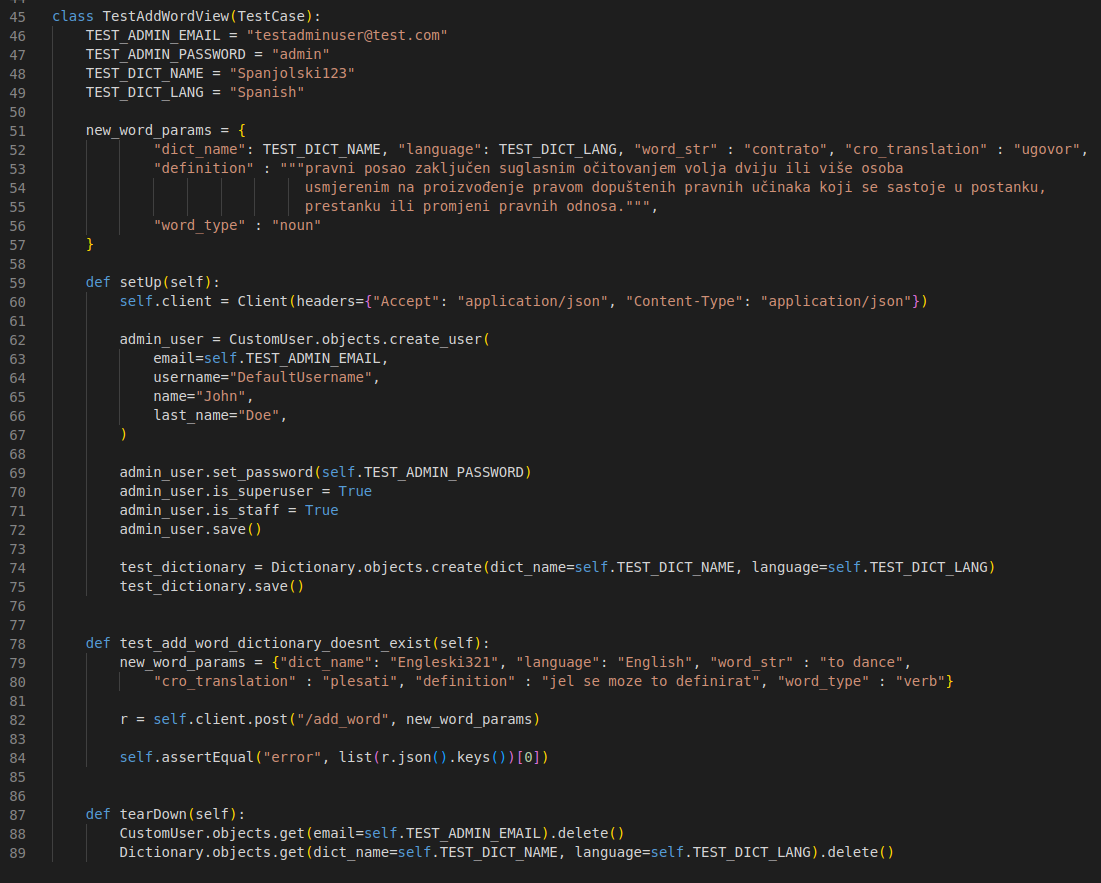
\includegraphics[width=\textwidth]{slike/test_add_word_dictionary_doesnt_exist.png}
				\caption{Ispitivanje dodavanja nove riječi u nepostojeći rječnik}
				\label{fig:test_add_word_dictionary_doesnt_exist}
			\end{figure}
		
			
			\eject
			
			
			\noindent{\textbf{Ispitivanje generiranja pitanja za način učenja odabirom točnog prijevoda}}\\
			\noindent{\textbf{Ulaz}: -\\\textbf{Očekivani izlaz:} generirano pitanje za način učenja odabirom točnog prijevoda\\\textbf{Opis ispitnog slučaja:} ispituje se generiranje pitanja za način učenja odabirom točnog prijevoda. Potrebno je izgenerirati pitanje, točan odgovor i netočne odgovore.
			}
			
			\begin{figure}[H]
				\centering
				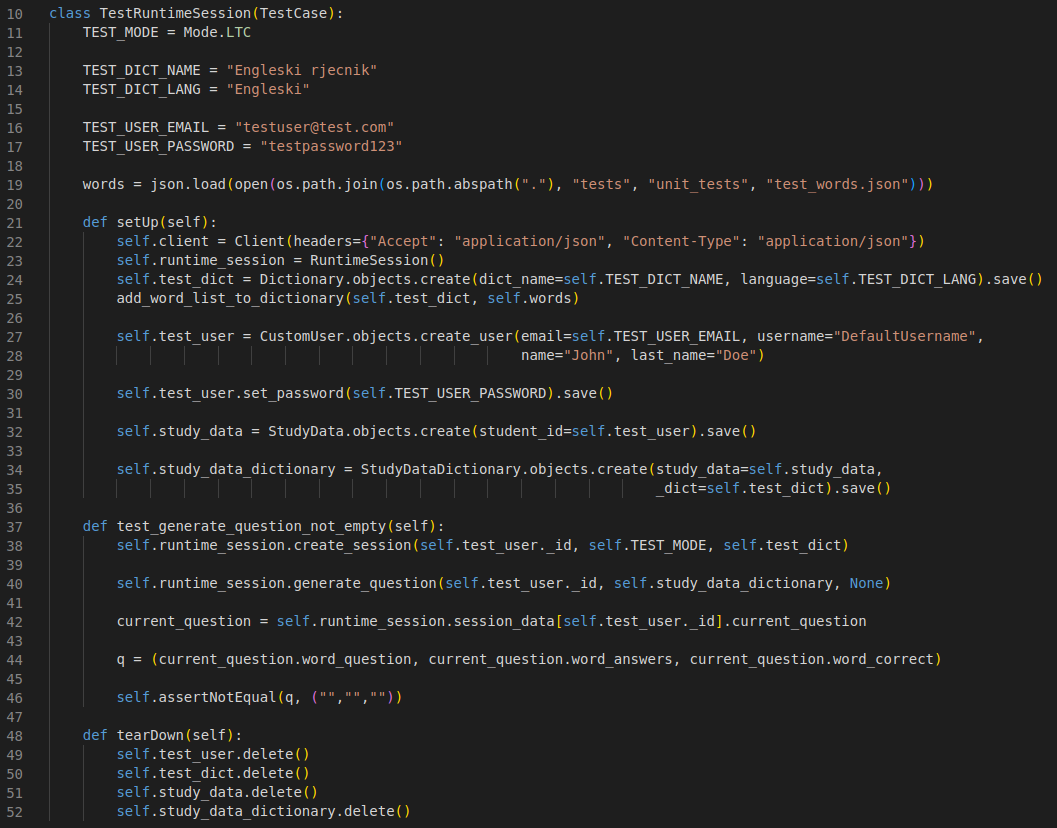
\includegraphics[width=\textwidth]{slike/test_generate_question_not_empty.png}
				\caption{Ispitivanje generiranja pitanja za način učenja odabirom točnog prijevoda}
				\label{fig:test_generate_question_not_empty}
			\end{figure}
			
			
			\eject
		

			\noindent{\textbf{Ispitivanje prijave korisnika u sustav}}\\
			\noindent{\textit{prvi dio ispitnog slučaja}}\\
			\noindent{\textbf{Ulaz}: ispravni email korisnika koji se želi prijaviti, ispravna lozinka\\\textbf{Očekivani izlaz:} uspješna prijava\\\textbf{Opis ispitnog slučaja:} ispituje se ispravnost odgovora funkcionalnosti prijave korisnika u sustav na situaciju u kojoj su uneseni ispravni podaci korisnika
			}\\
		
			\noindent{\textit{drugi dio ispitnog slučaja}}\\
			\noindent{\textbf{Ulaz}: ispravni email korisnika koji se želi prijaviti, neispravna lozinka korisnika\\\textbf{Očekivani izlaz:} neuspješna prijava\\\textbf{Opis ispitnog slučaja:} ispituje se ispravnost odgovora funkcionalnosti prijave korisnika u sustav na situaciju u kojoj je korisnik unio pogrešnu lozinku
			}
			
			\begin{figure}[H]
				\centering
				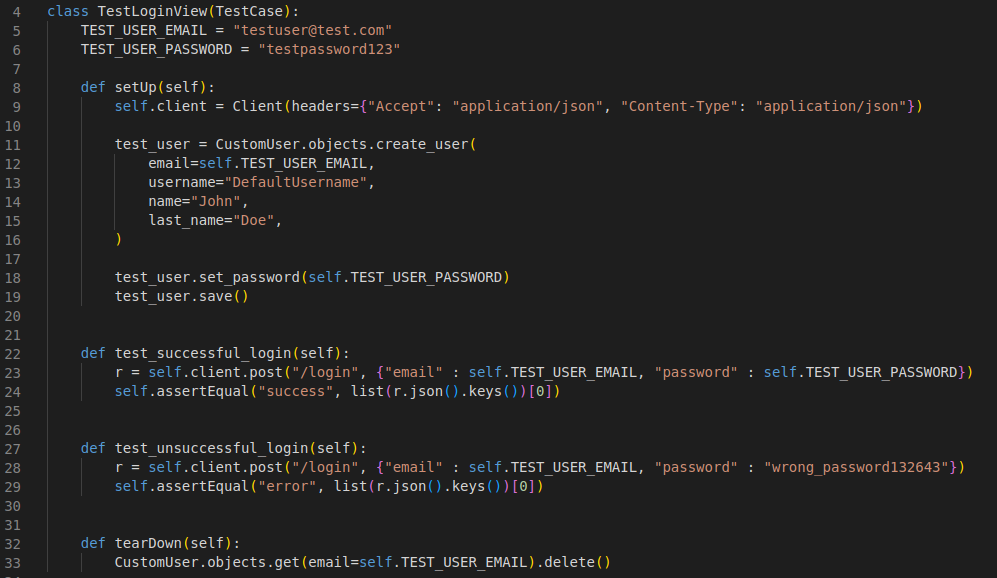
\includegraphics[width=\textwidth]{slike/test_login_view.png}
				\caption{Ispitivanje prijave korisnika u sustav}
				\label{fig:test_login_view}
			\end{figure}
			
			
			\eject
			
			
			\subsection{Ispitivanje sustava}
			
			\noindent{Ispitivanje sustava provedeno je korištenjem Selenium WebDrivera unutar alata za jedinično testiranje koje omogućuje radni okvir Django. Većina testova koji su prikazani u nastavku zahtijevaju da se prije izvršavanja glavnog dijela testa izvrši prijava u sustav. Na slici \ref{fig:login_function_selenium} je prikazana funkcija koja izvodi prijavu u sustav i koju pozivaju testovi. Funkcija "login" nije priložena uz izvorne kodove ispitnih slučajeva, no podrazumijeva se da postoji i da ju je moguće pozivati. Rezultati izvođenja ispitnih slučajeva prikazani su na slici \ref{fig:test_results_selenium}.}
			
			\begin{figure}[H]
				\centering
				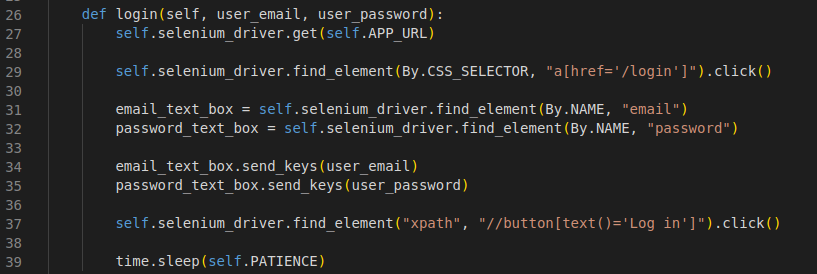
\includegraphics[width=\textwidth]{slike/login_function_selenium.png}
				\caption{Funkcija "login" koja prijavljuje korisnika u sustav}
				\label{fig:login_function_selenium}
			\end{figure}			
			
			\begin{figure}[H]
				\centering
				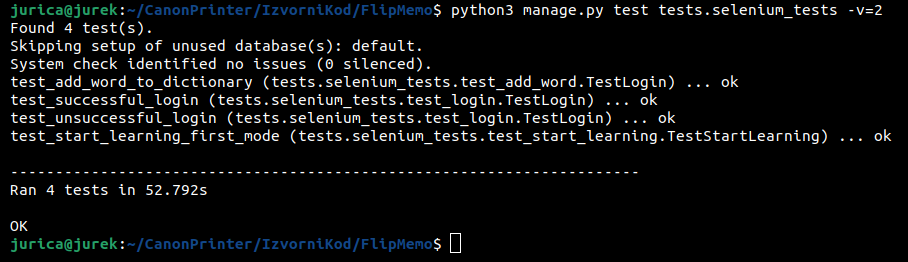
\includegraphics[width=\textwidth]{slike/test_results_selenium.png}
				\caption{Rezultati izvođenja ispitnih slučajeva}
				\label{fig:test_results_selenium}
			\end{figure}			
			
			\eject
			
			\noindent{\textbf{Ispitivanje dodavanja nove riječi u rječnik}}\\
			\noindent{\textbf{Ulaz}: podaci o novoj riječi koja se želi dodati u rječnik, rječnik u koji se riječ dodaje\\\textbf{Očekivani izlaz:} riječ nakon dodavanja postoji i nalazi se u odabranom rječniku\\\textbf{Opis ispitnog slučaja:} test simulira administratora koji prvo dodaje riječ u odabrani rječnik, a zatim pregledava da li mu se u odabranom rječniku prikazuje riječ nakon dodavanja
			}

			\begin{figure}[H]
				\centering
				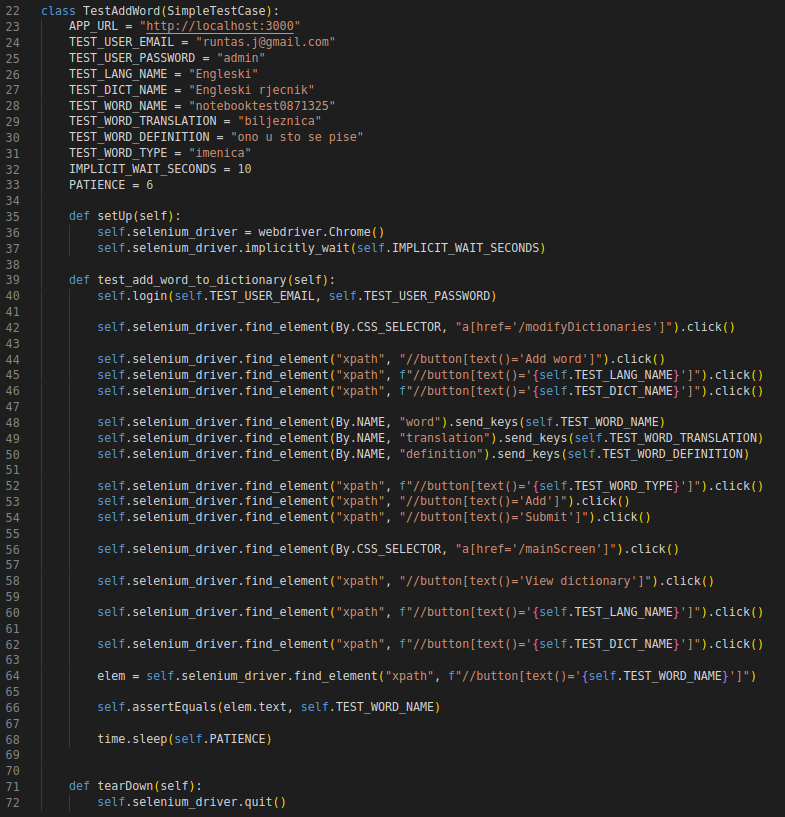
\includegraphics[width=\textwidth]{slike/test_add_word_to_dictionary.png}
				\caption{Ispitivanje dodavanja nove riječi u rječnik}
				\label{fig:test_add_word_to_dictionary}
			\end{figure}
			
			
			\eject 
			
			\noindent{\textbf{Ispitivanje pokretanja učenja u načinu učenja odabirom točnog odgovora}}\\
			\noindent{\textbf{Ulaz}: jezik rječnika iz kojeg se želi učiti, rječnik iz kojeg se želi učiti\\\textbf{Očekivani izlaz:} korisnik je preusmjeren na stranicu na kojoj se nalazi kviz sa načinom učenja odabirom točnog odgovora\\\textbf{Opis ispitnog slučaja:} test simulira korisnika koji odabire jezik i rječnik te način učenja odabirom točnog odgovora i pokreće učenje
			}
			
			\begin{figure}[H]
				\centering
				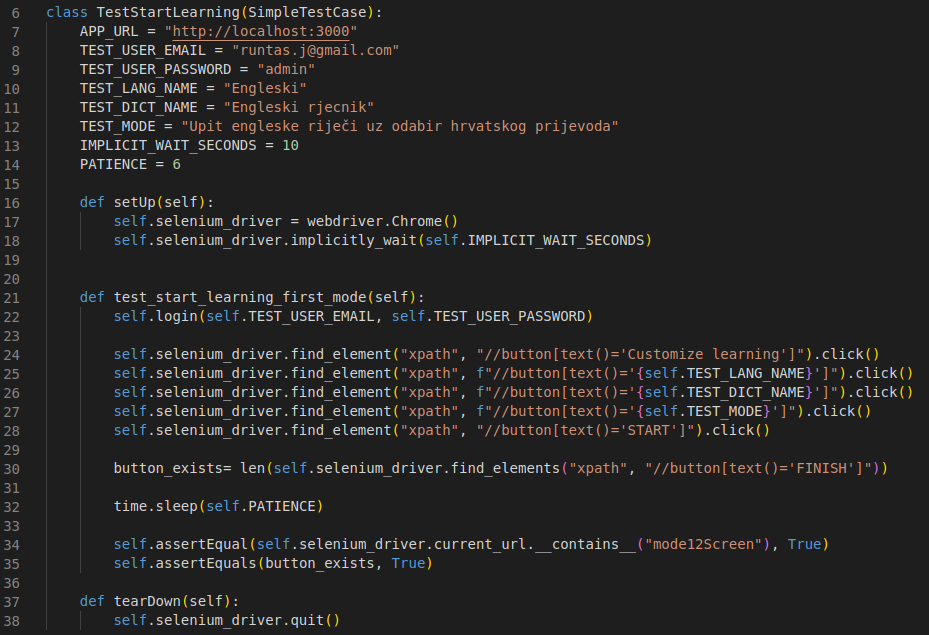
\includegraphics[width=\textwidth]{slike/test_start_learning_first_mode}
				\caption{Ispitivanje pokretanja učenja u načinu učenja odabirom točnog odgovora}
				\label{fig:test_start_learning_first_mode}
			\end{figure}
			
			
			\eject 
			
			\noindent{\textbf{Ispitivanje ispravne prijave u sustav}}\\
			\noindent{\textbf{Ulaz}: ispravna email adresa i lozinka korisnika\\\textbf{Očekivani izlaz:} korisnik je uspješno prijavljen u sustav i preusmjeren na početnu stranicu\\\textbf{Opis ispitnog slučaja:} test simulira korisnika koji se prijavljuje u sustav sa ispravnim podacima
			}
			
			\begin{figure}[H]
				\centering
				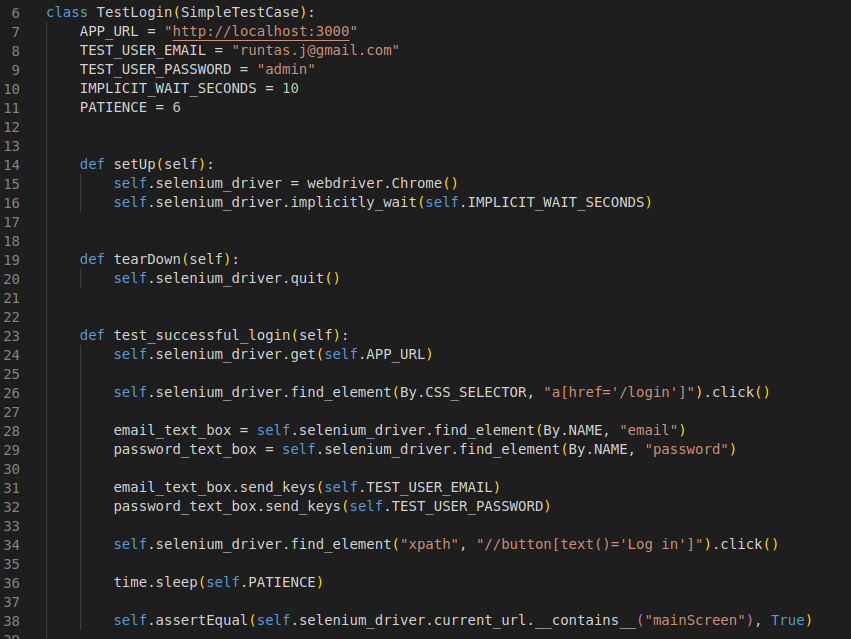
\includegraphics[width=\textwidth]{slike/test_successful_login}
				\caption{Ispitivanje ispravne prijave u sustav}
				\label{fig:test_successful_login}
			\end{figure}
			
			
			\eject 
			
			
			\noindent{\textbf{Ispitivanje neispravne prijave u sustav}}\\
			\noindent{\textbf{Ulaz}: ispravna email adresa i neispravna lozinka korisnika\\\textbf{Očekivani izlaz:} korisniku se pojavljuje upozorenje da je unio neispravnu email adresu i/ili lozniku\\\textbf{Opis ispitnog slučaja:} test simulira korisnika koji se prijavljuje u sustav sa ispravnom email adresom i neispravnom lozinkom
			}
			
			\begin{figure}[H]
				\centering
				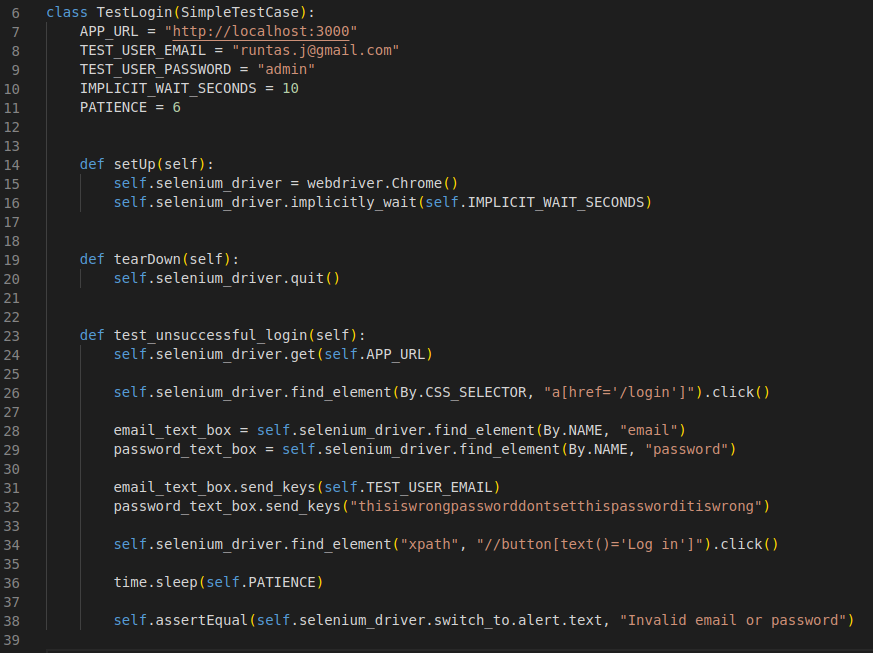
\includegraphics[width=\textwidth]{slike/test_unsuccessful_login}
				\caption{Ispitivanje neispravne prijave u sustav}
				\label{fig:test_unsuccessful_login}
			\end{figure}
			
			
			\eject 
		
		
		\section{Dijagram razmještaja}
			
			\noindent{Na dijagramu razmještaja je prikazana topologija sustava i odnos programskih artefakata.}
			
			\indent{Web aplikacija se kao programski artefakt izvršava u Heroku Dyno spremniku koji je vrsta Linux spremnika proširen sa raznim mogućnostima upravljanja koje nudi Heroku platforma.}
			
			\indent{Aplikacija ovisi o bazi podataka koja se nalazi na MongoDB Atlas poslužitelju. Pristup i rad s bazom podataka omogućuje usluga MongoDB Atlas Cluster. Za potrebe dohvata podataka o riječima aplikacija koristi Datamuse API, a za potrebe generiranja zvučnih datoteka izgovora riječi koristi Google Text-to-Speech API.	
			}
			
			\indent{Korisnici (učenici i administratori riječi) koriste web preglednik kako bi pristupili web aplikaciji. Arhitektura sustava bazira se na arhitekturi "klijent - poslužitelj". Komunikacija između korisničkog računala i poslužitelja odvija se preko HTTPS veze.}
			
			\begin{figure}[H]
				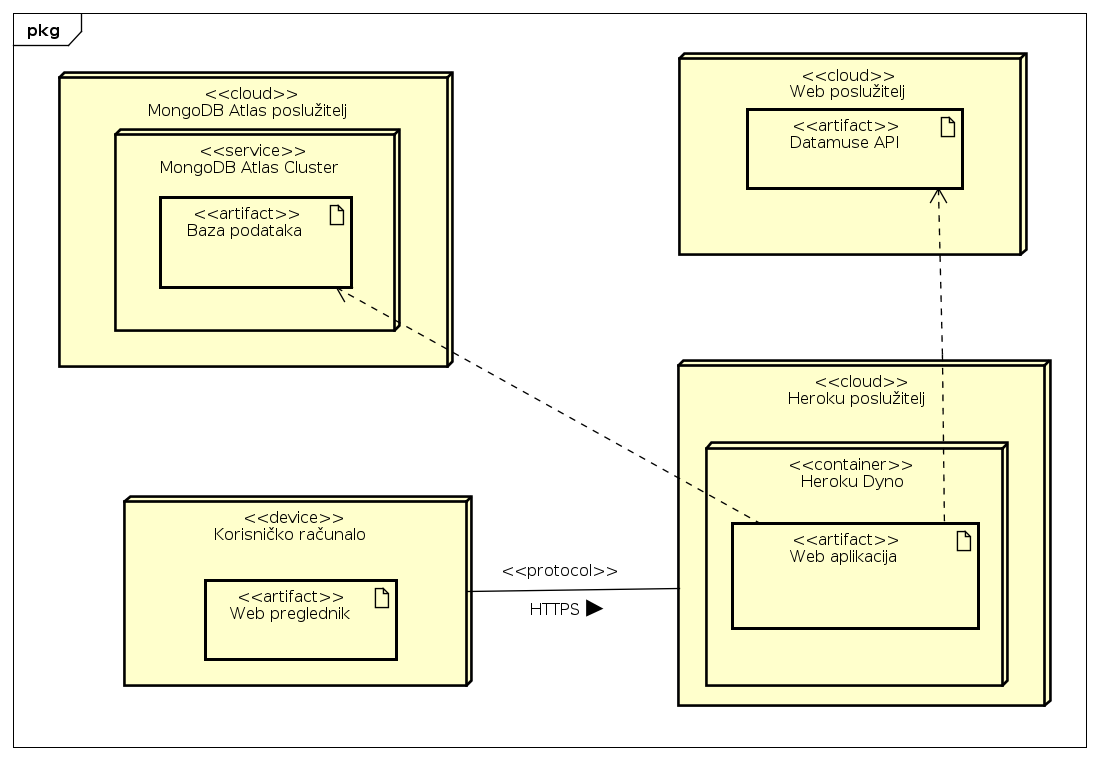
\includegraphics[width=\textwidth]{dijagrami/dijagram_razmjestaja.png} %veličina u odnosu na širinu linije
				\caption{Dijagram razmještaja}
				\label{fig:Dijagram_razmjestaja} %label mora biti drugaciji za svaku sliku
			\end{figure}
			
			\eject 
		
		\section{Upute za puštanje u pogon}
			
			\noindent{\textbf{Konfiguracija poslužitelja baze podataka}}\\
			\noindent{MongoDB Atlas nudi mogućnosti korištenja MongoDB baze podataka na udaljenom poslužitelju, za što je potreban MongoDB korisnički račun. S uspješno stvorenim računom moguće je napraviti novi "Deployment" koji će sadržavati sve baze podataka (eng. cluster). Prilikom stvaranja novog deploymenta odabire se pružatelj usluge poslužitelja i fizička lokacija samog poslužitelja na kojem će se cluster nalaziti (slika \ref{fig:Odabir poslužitelja BP-a}).}
			
			\begin{figure}[H]
				\centering
				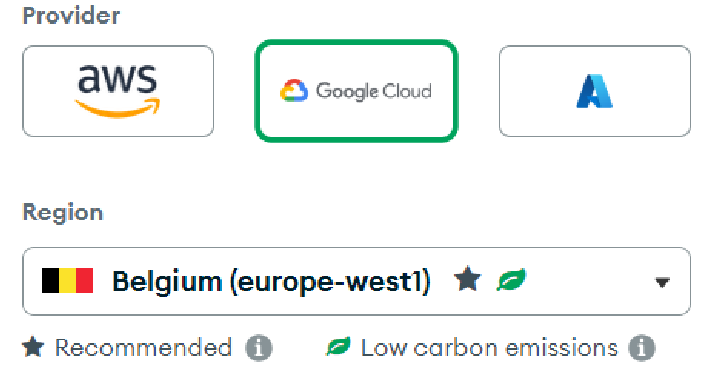
\includegraphics[width=0.5\textwidth]{slike/bp1.png}
				\caption{Odabir poslužitelja baze podataka}
				\label{fig:Odabir poslužitelja BP-a}
			\end{figure}
			
			\noindent{\textbf{Konfiguracija baze podataka}}\\
			\noindent{Na novostvorenom poslužitelju možemo pokrenuti novu bazu podataka, ali prvo je potrebno spojiti se na cluster. Na cluster se spajamo s nekim korisnikom koji ima određene priviligije. Budući da smo cluster tek stvorili, MongoDB će nas prvi prvom povezivanju na cluster tražiti ime i lozinku novog korisnika koji će imati "atlasAdmin" privilegije. Atlas, kao razinu sigurnosti, dopušta spajanje na cluster samo preko potvrđenih IP-adresa, zato je nužno dodati IP-adresu poslužitelja aplikacije kao potvrđenu. Na Security $\rightarrow$ Network Access $\rightarrow$ + ADD IP ADDRESS (slika \ref{fig:Dodavanje IP}) upisujemo IP-adresu poslužitelja aplikacije.}
			
			\begin{figure}[H]
				\centering
				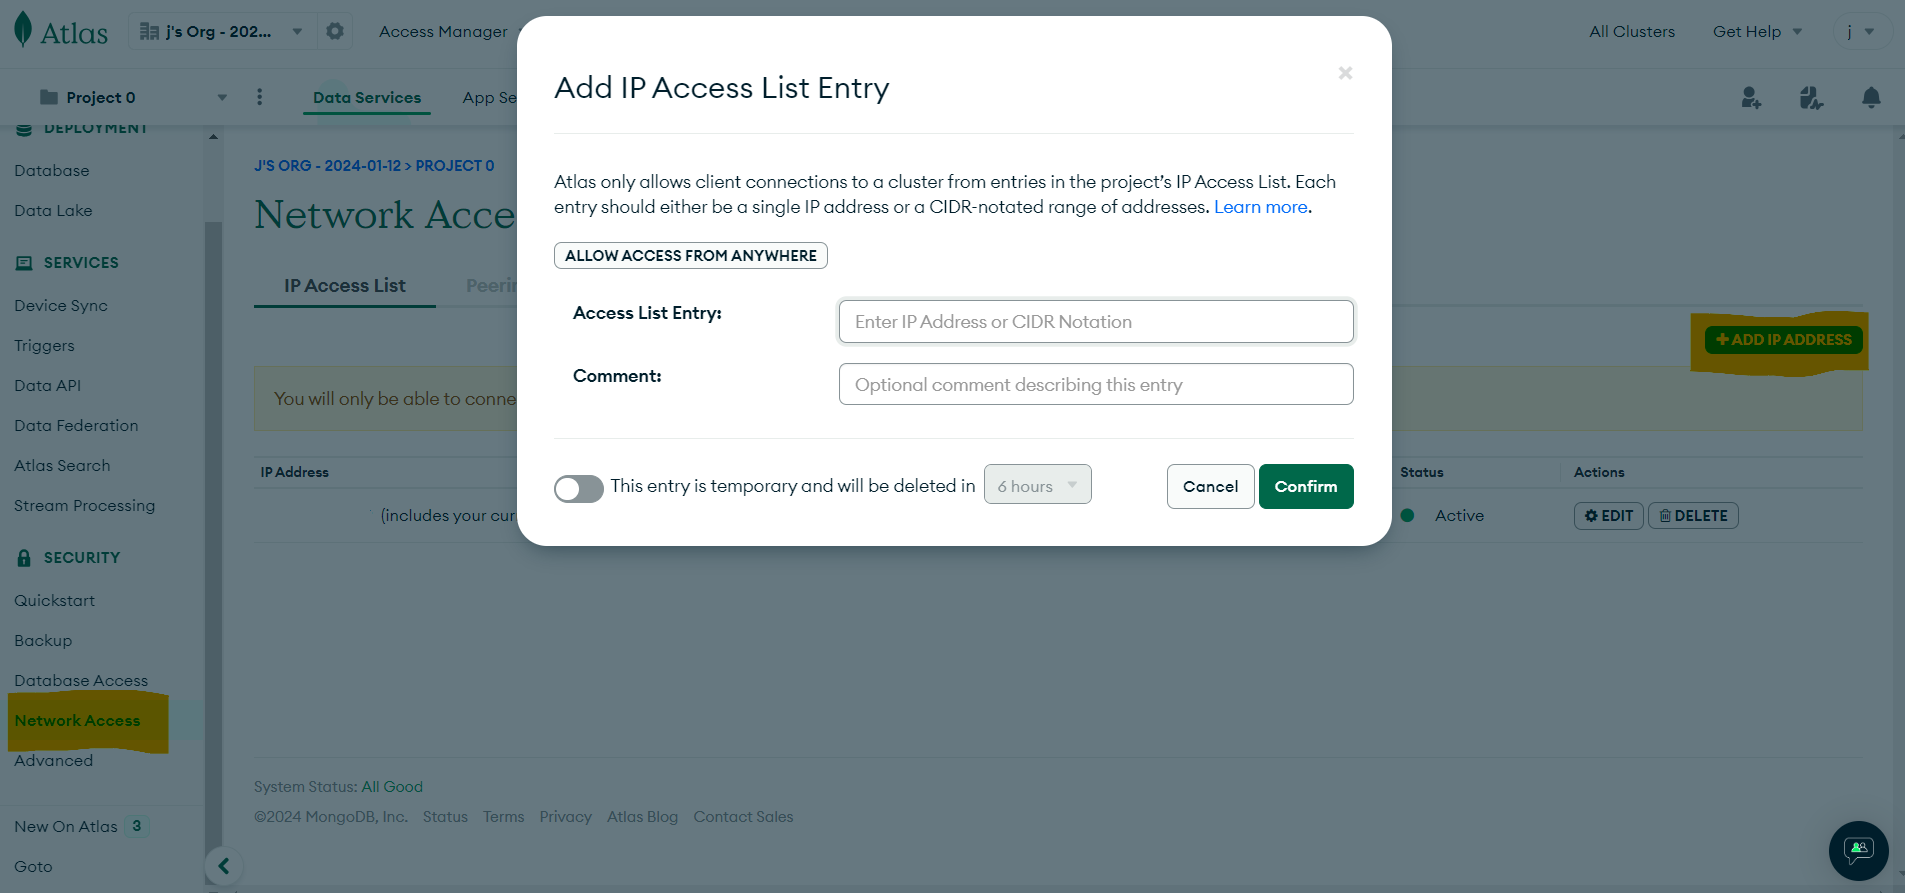
\includegraphics[width=\textwidth]{slike/dodavanje_ip.png}
				\caption{Postupak dodavanja IP-adrese u listu potvrđenih}
				\label{fig:Dodavanje IP}
			\end{figure}
			
			\noindent{Aplikacija sada može pristupiti bazi podataka. Odlaskom na Deployment $\rightarrow$ Database $\rightarrow$ Collections $\rightarrow$ + Create Database stvaramo novu bazu podataka.} \\
			
			\noindent{\textbf{Konfiguracija Heroku poslužitelja}}\\
			\noindent{Nakon što se uspješno izradi Heroku korisnički račun, potrebno je stvoriti novu aplikaciju u "Dashboardu" klikom na "Create new app". Potrebno je upisati ime aplikacije, odabrati regiju i završiti stvaranje aplikacije klikom na "Create app". Forma za izradu aplikacije je prikazana na slici \ref{fig:StvaranjeAplikacije}}.
			
			
			\begin{figure}[H]
				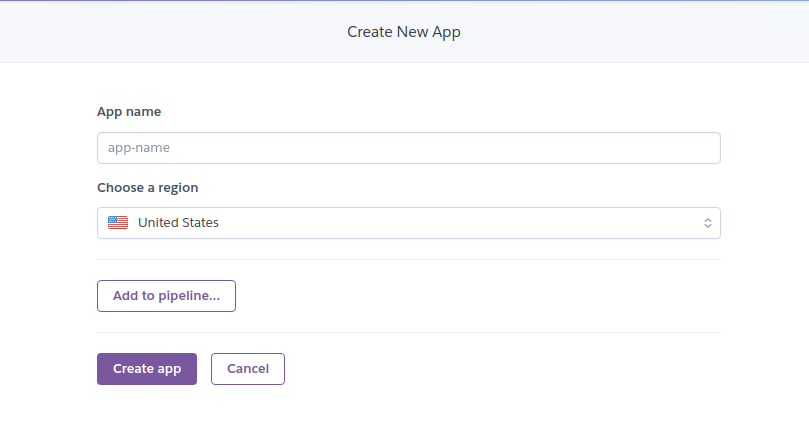
\includegraphics[width=\textwidth]{slike/stvaranjeAplikacije.png} %veličina u odnosu na širinu linije
				\caption{Stvaranje nove aplikacije}
				\label{fig:StvaranjeAplikacije} %label mora biti drugaciji za svaku sliku
			\end{figure}
		
			
			\indent{Nakon izrade aplikacije potrebno je podesiti konfiguraciju u "Settings" dijelu aplikacije kao što je prikazano na slikama \ref{fig:podesi1} i \ref{fig:podesi2}. "DB CONNECTION STRING" se dobije prilikom konfiguracije baze podataka i služi aplikaciji za pristup bazi podataka, a "SECRET KEY" je tajni ključ čija će vrijednost ovisiti o konkretnom projektu, Django ga interno koristi za potrebe hashiranja. Moguće je i podesiti ostale parametre po potrebi.}\\
			\indent{Potrebno je i dodati "Buildpack" za Node.js i Python s obzirom da aplikacija koristi programski jezik Python za backend, a React za frontend. "Buildpackovi" služe za instaliranje svega onoga što je potrebno da bi se aplikacija mogla pokrenuti na Heroku poslužitelju.}
			
			
			\begin{figure}[H]
				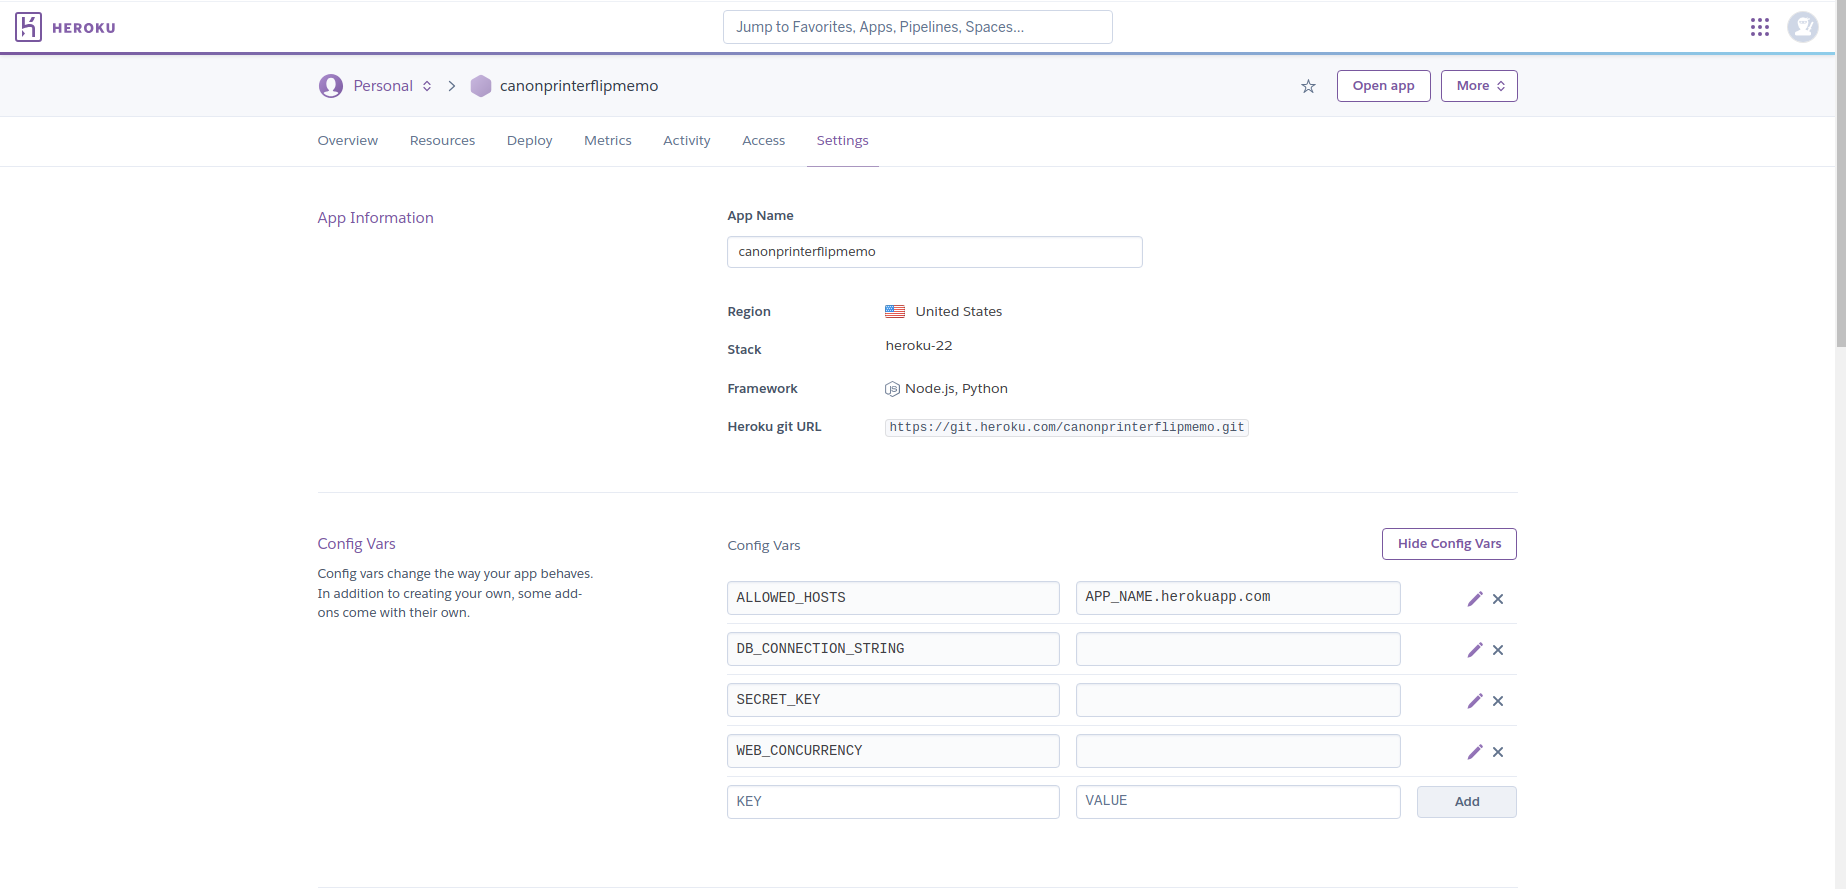
\includegraphics[width=\textwidth]{slike/podesi1.png} %veličina u odnosu na širinu linije
				\caption{Konfiguracija konfiguracijski varijabli}
				\label{fig:podesi1} %label mora biti drugaciji za svaku sliku
			\end{figure}
		
			\begin{figure}[H]
				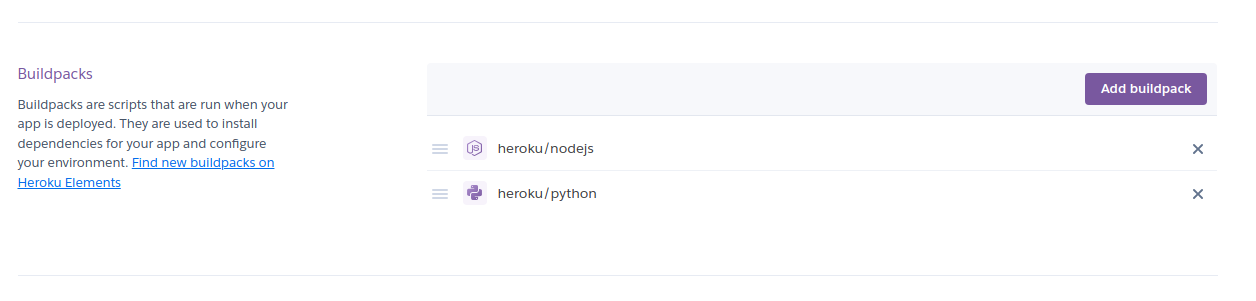
\includegraphics[width=\textwidth]{slike/podesi2.png} %veličina u odnosu na širinu linije
				\caption{Konfiguracija "Buildpackova"}
				\label{fig:podesi2} %label mora biti drugaciji za svaku sliku
			\end{figure}
		
			\noindent{\textbf{Organizacija strukture projekta za puštanje u pogon}}\\
			\noindent{Za potrebe puštanje aplikacije u pogon pomoću Heroku usluge, potrebno je organizirati strukturu projekta odnosno izvornog koda u onakvu strukturu kakvu Heroku očekuje prilikom prijenosa izvornog koda na Heroku poslužitelj. Reorganizacija strukture projekta većim dijelom uključuje reorganizaciju postojeće hijerarhije direktorija, no potrebno je dodati i neke konfiguracijske datoteke što je opisano u nastavku.}\\
			\indent{Na slici \ref{fig:organizacijaKoda} je prikazan primjer strukture projekta kakvu očekuje Heroku. "FlipMemo", "main" i "users" su mape iz Django dijela aplikacije, a "src", "public" iz React dijela aplikacije. Bitno je da sve te mape budu na istoj razini u glavnom direktoriju "CanonPrinter". "staticfiles" mapa je trenutno prazna, no u nju se prilikom puštanja u pogon spremaju razne datoteke nakon što se odradi "build" na Heroku poslužitelju.}
			
			\begin{figure}[H]
				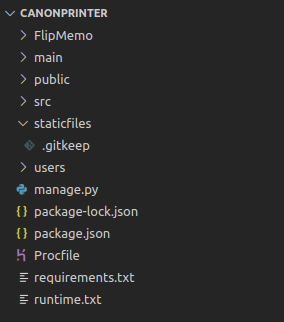
\includegraphics[width=\textwidth]{slike/organizacijaKoda.png} %veličina u odnosu na širinu linije
				\caption{Struktura projekta za puštanje aplikacije u pogon}
				\label{fig:organizacijaKoda} %label mora biti drugaciji za svaku sliku
			\end{figure}
		
			\noindent{"manage.py", "package.json" i "package-lock.json" su datoteke koje postoje i prije reorganizacije strukture projekta, a vezanu su uz Django i React dok su "Procfile", "requirements.txt" i "runtime.txt" konfiguracijske datoteke koje Heroku očekuje da postoje u projektu i moraju se dodati prije puštanja aplikacije u pogon. Sadržaj konfiguracijskih datoteke prikazan je na slikama \ref{fig:konf1}, \ref{fig:konf2}, \ref{fig:konf3}. 
			
			\begin{figure}[H]
				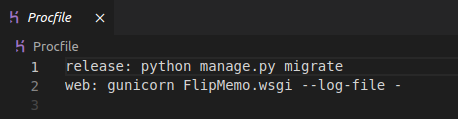
\includegraphics[width=\textwidth]{slike/konf1.png} %veličina u odnosu na širinu linije
				\caption{Procfile}
				\label{fig:konf1} %label mora biti drugaciji za svaku sliku
			\end{figure}
		
			\begin{figure}[H]
				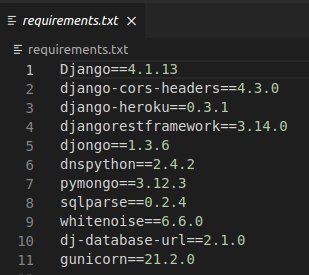
\includegraphics[width=\textwidth]{slike/konf2.png} 	%veličina u odnosu na širinu linije
				\caption{requirements.txt}
				\label{fig:konf2} %label mora biti drugaciji za svaku sliku
			\end{figure}
		
			Svaka konfiguracijska datoteka sadrži konfiguracijske parametre koji su potrebni prilikom puštanja aplikacije u pogon, npr. verzije svih potrebnih biblioteka koje je potrebno instalirati, verziju programskog jezika Python i sl. Za detalje o tome kako Heroku koristi te konfiguracijske datoteke upućujemo na službenu dokumentaciju\footnote{\url{https://devcenter.heroku.com/categories/reference}}.}
	
			\begin{figure}[H]
				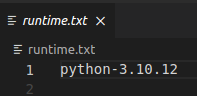
\includegraphics[width=\textwidth]{slike/konf3.png} %veličina u odnosu na širinu linije
				\caption{runtime.txt}
				\label{fig:konf3} %label mora biti drugaciji za svaku sliku
			\end{figure}
		
			\noindent{\textbf{Puštanje aplikacije u pogon korištenjem Heroku Git}}\\
			\noindent{Nakon provedenih svih potrebnih prethodno opisanih koraka, aplikacije se može pustiti u pogon na Heroku poslužitelj na više načina. Ovdje prikazujemo način puštanja aplikacije u pogon korištenjem Heroku Gita. Potrebno je instalirati Heroku CLI koji omogućuje rad sa Heroku korištenjem komandne linije \footnote{\url{https://devcenter.heroku.com/articles/heroku-cli}}.}\\
			\indent{Nakon što je Heroku CLI uspješno instaliran za odgovarajuću platformu, potrebno je provesti postupak prijenosa izvornog koda projekta na Heroku poslužitelj kojim se automatski pokreće i proces izgradnje i puštanja aplikacije u pogon. Slika \ref{fig:herokucli} prikazuje sve potrebne korake kod rada sa Heroku CLI. Aplikacija je nakon provedenih koraka dostupna na poveznici koju je izgenerirao proces puštanja aplikacije u pogon. Moguće je i zadati svoju vlastitu domenu na kojoj će aplikacija biti dostupna što je prikazano na slici \ref{fig:customDomena}}.
			
			\begin{figure}[H]
				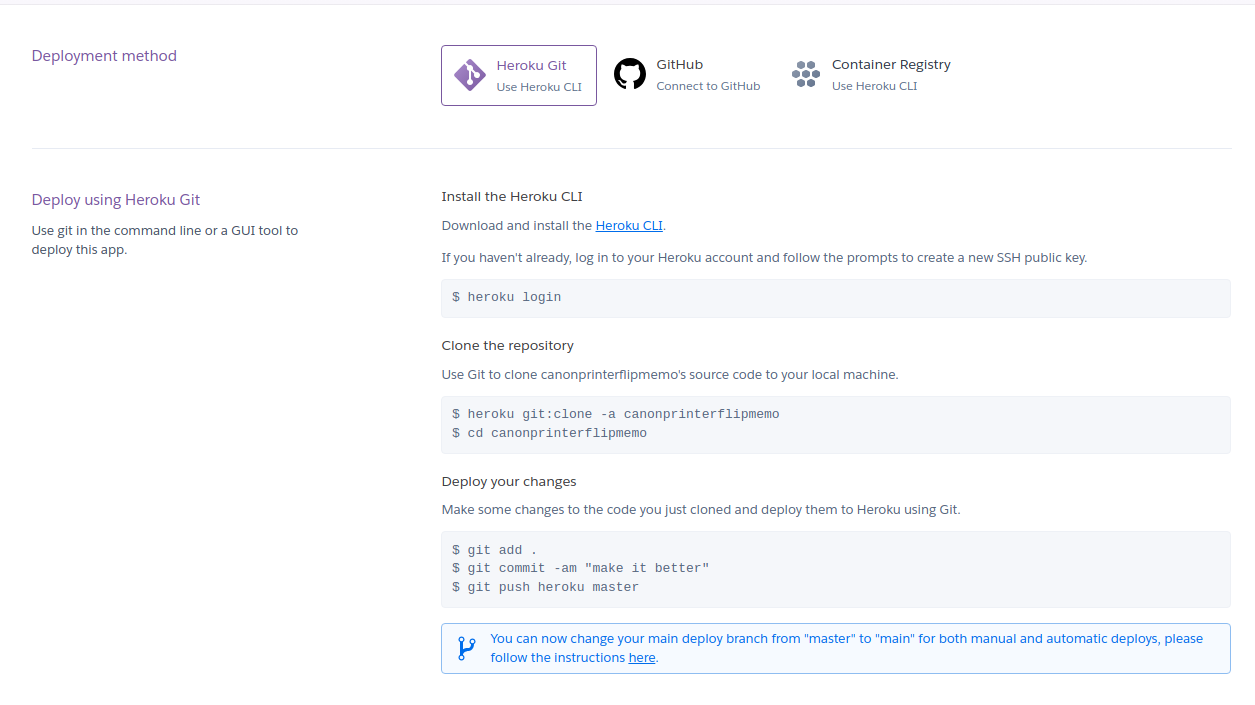
\includegraphics[width=\textwidth]{slike/herokucli.png} %veličina u odnosu na širinu linije
				\caption{Puštanje aplikacije u u pogon korištenjem Heroku CLI}
				\label{fig:herokucli} %label mora biti drugaciji za svaku sliku
			\end{figure}
		
			\begin{figure}[H]
				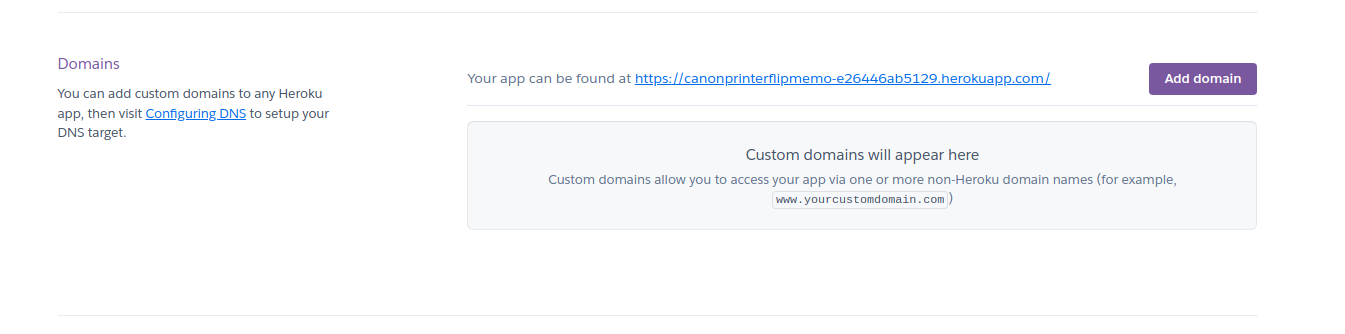
\includegraphics[width=\textwidth]{slike/customDomena.png} %veličina u odnosu na širinu linije
				\caption{Dio postavka za podešavanje domene aplikacije}
				\label{fig:customDomena} %label mora biti drugaciji za svaku sliku
			\end{figure}
			
			\eject 